\documentclass[tikz]{standalone}

\usepackage{tikz}
\usetikzlibrary{calc}


\newcommand\term[2]{\node[below]at(#1){$#2$};}

\begin{document}
% macro for inputting terminal nodes

%
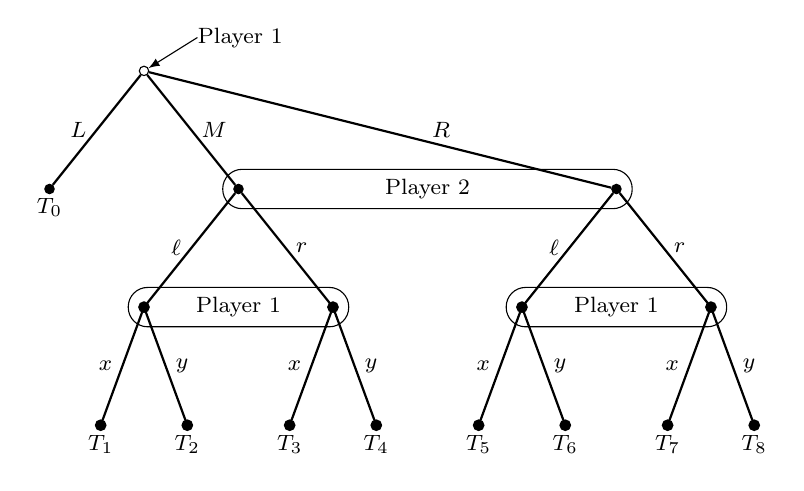
\begin{tikzpicture}[font=\footnotesize,edge from parent/.style={draw,thick}]
% Two node styles: solid and hollow
\tikzstyle{solid node}=[circle,draw,inner sep=1.2,fill=black];
\tikzstyle{hollow node}=[circle,draw,inner sep=1.2];
% Specify spacing for each level of the tree
\tikzstyle{level 1}=[level distance=15mm,sibling distance=12mm]
\tikzstyle{level 2}=[level distance=15mm,sibling distance=24mm]
\tikzstyle{level 3}=[level distance=15mm,sibling distance=11mm]
% The Tree
\node(0)[hollow node]{}
child{node[solid node]{}edge from parent node[left]{$L$}}
child{node[solid node]at +(\tikzsiblingdistance,0){}
child{node[solid node]{}
child{node[solid node]{}edge from parent node[left]{$x$}}
child{node[solid node]{}edge from parent node[right]{$y$}}
edge from parent node[left]{$\ell$}
}
child{node[solid node]{}
child{node[solid node]{}edge from parent node[left]{$x$}}
child{node[solid node]{}edge from parent node[right]{$y$}}
edge from parent node[right]{$r$}
}
edge from parent node[right]{$M$}
}
child[sibling distance=5*\tikzsiblingdistance]{node[solid node]{}
child{node[solid node]{}
child{node[solid node]{}edge from parent node[left]{$x$}}
child{node[solid node]{}edge from parent node[right]{$y$}}
edge from parent node[left]{$\ell$}
}
child{node[solid node]{}
child{node[solid node]{}edge from parent node[left]{$x$}}
child{node[solid node]{}edge from parent node[right]{$y$}}
edge from parent node[right]{$r$}
}
edge from parent node[right,xshift=15]{$R$}
};
% information sets
\draw[rounded corners=7]($(0-2)+(-.2,.25)$)rectangle($(0-3)+(.2,-.25)$);
\draw[rounded corners=7]($(0-2-1)+(-.2,.25)$)rectangle($(0-2-2)+(.2,-.25)$);
\draw[rounded corners=7]($(0-3-1)+(-.2,.25)$)rectangle($(0-3-2)+(.2,-.25)$);
% specifying movers
\draw[draw,<-,>=latex](0)--(32:8mm)node[right,inner sep=0]{Player 1};
\node at ($.5*(0-2)+.5*(0-3)$) {Player 2};
\node at ($.5*(0-2-1)+.5*(0-2-2)$) {Player 1};
\node at ($.5*(0-3-1)+.5*(0-3-2)$) {Player 1};
% specifying terminal nodes
\newcounter{tnode}
\setcounter{tnode}{0}
\term{0-1}{T_\arabic{tnode}}
\foreach \x in {2,3}
\foreach \y in {1,2}
\foreach \z in {1,2}
\stepcounter{tnode}
\term{0-\x-\y-\z}{T_\arabic{tnode}};
\end{tikzpicture}
\end{document}